\section{数理统计的基本概念}
\subsection{总体\&样本}
\begin{enumerate}
	\item 总体: 数理统计中所研究对象的某项指标$X$的全体称为总体。
	\item 样本: 如果$X_1, X_2, \dots, X_n$相互独立且都与总体$X$同分布,则称$X_1, X_2, \dots, X_n$为来自总体的简单随机样本,简称为样本。\\
	其中,$n$为样本容量,样本的具体观测值$x_1, x_2, \dots, x_n$为样本值,或称总体$X$的$n$个独立观测值。
	\begin{enumerate}
		\item 若总体$X$的分布为$F(x)$,则样本$X_1, X_2, \dots, X_n$的分布为
		\begin{equation}
			F_n(x_1, x_2, \dots, x_n) = \prod_{i=1}^{n}F(x_i)
		\end{equation}

		\item 若总体$X$的概率密度为$f(x)$,则样本$x_1, x_2, \dots, x_n$的概率密度为
		\begin{equation}
			f_n(x_1, x_2, \dots, x_n) = \prod_{i=1}^{n}f(x_i)
		\end{equation}
		\item 若总体$X$的概率分布为$P(X=a_j)=p_j, \quad j = 1,2, \dots$,则样本$X_1, X_2, \dots, X_n$的概率分布为
		\begin{equation}
			P(X_1=x_1, X_2=x_2, \dots, X_n=x_n) = \prod_{i=1}^{n}P(X_i = x_i)
		\end{equation}
		所以,在逻辑回归中,似然函数$L(\theta)$可以写成各个概率的乘积:
		\begin{equation}
			L(\theta)=\prod_{i=1}^{m}p(y^{(i)}|x^{(i)}; \theta)
		\end{equation}
		在机器学习中,每个数据点$(x^{(i)},y^{(i)})$就是总体中的一个个体(满足独立同分布)。所以上式中,乘积的上下限对应的是样本,故应为$i=1 \to m$
	\end{enumerate}
\end{enumerate}

\subsection{统计量}
\begin{enumerate}
	\item 统计量: 样本$X_1, X_2, \dots, X_n$的不含未知参数的函数$T = T(X_1, X_2, \dots, X_n)$称为统计量。
	\item 作为随机样本的函数,统计量本身也是一个随机变量。
	\item 若$x_1, x_2, \dots, x_n$是样本$X_1, X_2, \dots, X_n$的样本值,则数值$T(x_1, x_2, \dots, x_n)$是统计量$T = T(X_1, X_2, \dots, X_n)$的观测值。
	% \item 在迷你梯度下降中的Cost Function应该就是个统计量,$J(\theta)=\frac{1}{2}\sum_{i=1}^{m}\left[h_\theta(x^{(i)}) - y^{(i)}\right]^2$,其中,$\sum_{i=1}^{m}$就是这个$T${\color{red}{(正确性待查)}}
	\item 在指数分布族中,$T(y)$是个充分统计量
\end{enumerate}

\subsection{样本的数字特征}
设$X_1, X_2, \dots, X_n$是来自总体$X$的样本,则
\begin{enumerate}
	\item 样本均值
	\begin{equation}
		\bar X = \frac{1}{n}\sum_{i=1}^{n} X_i
	\end{equation}

	\item 样本方差
	\begin{equation}
		S^2 = \frac{1}{n-1}\sum_{i=1}^{n}(X_i - \bar X)^2
	\end{equation}
	样本标准差
	\begin{equation}
		S = \sqrt{\frac{1}{n-1}\sum_{i=1}^{n}(X_i - \bar X)^2}
	\end{equation}

	\item 样本$k$阶原点距
	\begin{equation}
		A_k = \frac{1}{n}\sum_{i=1}^{n}X_i^k, \quad k = 1, 2; \quad A_1 = \bar X
	\end{equation}

	\item 样本$k$阶中心距
	\begin{equation}
		B_k = \frac{1}{n}\sum_{i=1}^{n}(X_i - \bar X)^k, \quad k = 1, 2; \quad B_2 = \frac{n-1}{n}S^2 \neq S^2
	\end{equation}
\end{enumerate}

\subsection{样本的数字特征的性质}
\begin{enumerate}
	\item 若总体$X$具有数学期望$E(X)=\mu$,则
	\begin{equation}
		E(\bar X) = E(X) = \mu
	\end{equation}
	注意均值与期望的区别,均值针对的是样本(样本均值),期望针对的是事件(事件期望)。
	\item 若总体$X$具有方差$D(X)=\sigma^2$,则
	\begin{align}
		D(\bar X) &= \frac{1}{n}D(X) = \frac{\sigma^2}{n} \\
		E(S^2) &= D(X) = \sigma^2
	\end{align}
	\item 若总体$X$的$k$阶原点矩$E(X^k) = \mu_k, \quad k = 1, 2, \dots$存在,则当$n \to \infty$时:
	\begin{equation}
		\lim_{n\to \infty} \frac{1}{n}\sum_{i=1}^{n}X_i^k \xrightarrow{\quad P \quad} \mu_k, \quad k = 1, 2, \dots
	\end{equation}
\end{enumerate}

\subsection{常用统计抽样分布}
\subsubsection{$\chi^2$分布}
\begin{enumerate}
	\item $\chi^2$分布 \\
	若随机变量$X_1, X_2, \dots, X_n$相互独立且均服从标准正态分布$N(0,1)$,则称随机变量$\chi^2 = X_1^2+X_2^2+\dots+X_n^2$服从自由度为$n$的$\chi^2$分布,记做$\chi^2 \sim \chi^2(n)$
	\item $\chi^2$分布的性质 \\
	\begin{enumerate}
		\item $n$个相互独立的标准正态随机变量的平方和$\chi^2 = X_1^2+X_2^2+\dots+X_n^2$又称为$\chi^2(n)$的典型模式。
		\item 若$0<\alpha<1$,则称满足条件
		\begin{equation}
			P(\chi^2 > \chi_{\alpha}^{2}(n)) = \int_{\chi_{\alpha}^{2}(n)}^{+\infty}f(x)dx = \alpha
		\end{equation}
		的点为$\chi_{\alpha}^{2}(n)$为$\chi^2(n)$分布的上$\alpha$分位点。
		\begin{figure}[htbp]
			\centering
			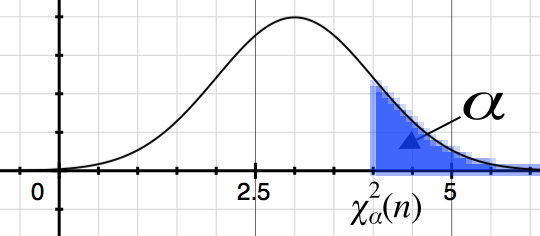
\includegraphics[scale=0.9]{contents/分位点}
			\caption{$\chi^2$分布分位点示例图}
		\end{figure}
		\item $E(\chi^2) = n$,$D(\chi^2)=2n$
		\item 若$\chi_1^2 \sim \chi^2(n_1)$,$\chi_2^2 \sim \chi^2(n_2)$,且$\chi_1^2$与$\chi_2^2$相互独立,则$\chi_1^2 + \chi_2^2 \sim \chi^2(n_1+n_2)$
	\end{enumerate}
\end{enumerate}

\subsubsection{$t$分布}
\begin{enumerate}
	\item $t$分布 \\
	若随机变量$X$与$Y$相互独立,且$X\sim N(0,1)$,$Y\sim \chi^2(n)$,则称随机变量
	\begin{equation}
		T = \frac{X}{\sqrt{\frac{Y}{n}}}
	\end{equation}
	服从自由度为$n$的$t$分布,记做$T \sim t(n)$

	\item $t$分布的性质
	\begin{enumerate}
		\item 满足$X,Y$相互独立,$X\sim N(0,1)$,$Y\sim \chi^2(n)$三个条件的$T = \frac{X}{\sqrt{\frac{Y}{n}}}$称为$t(n)$的典型分布
		\item $t$分布的概率密度$f(x)$是偶函数,即$f(x) = f(-x)$
		\item 当$n$充分大时,$t(n)$分布近似于$N(0,1)$分布
		\item 若$0<\alpha<1$,则称满足条件
		\begin{equation}
			P(T > t_{\alpha}(n)) = \int_{t_{\alpha}(n)}^{+\infty}f(x)dx = \alpha
		\end{equation}
		的点为$t_{\alpha}(n)$为$t(n)$分布的上$\alpha$分位点。
		\item 因为$t(n)$分布的概率密度为偶函数,故可知$t$分布的双侧$\alpha$分位点$t_{\frac{\alpha}{2}}(n)$,即
		\begin{equation}
			P\left(|T|>t_{\frac{\alpha}{2}}(n)\right) = \alpha
		\end{equation}
		\begin{figure}[htbp]
			\centering
			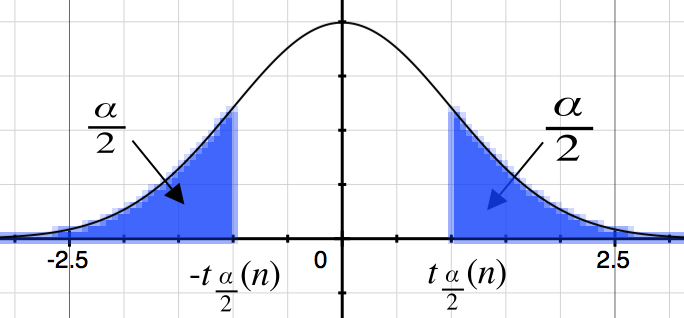
\includegraphics[scale=0.9]{contents/t分布分位点}
			\caption{$t$分布分位点示例图}
		\end{figure}
		如图可知,$t_{1-\alpha}(n) = -t_{\alpha}(n)$(将$\frac{\alpha}{2}$用$\alpha$代替,公式更好看)。
	\end{enumerate}
\end{enumerate}

\subsubsection{$F$分布}
\begin{enumerate}
	\item $F$分布 \\
	若随机变量$X$与$Y$相互独立,且$X\sim \chi^2(n_1)$,$Y\sim \chi^2(n_2)$,则称随机变量
	\begin{equation}
		F = \frac{\frac{X}{n_1}}{\frac{Y}{n_2}}
	\end{equation}
	服从自由度为$(n_1, n_2)$的$F$分布,记做$F \sim F(n_1, n_2)$,其中,$n_1, n_2$分别称为第一自由度和第二自由度
	\item $F$分布的性质 \\
	\begin{enumerate}
		\item 满足$X,Y$独立,$X\sim \chi^2(n_1)$,$Y\sim \chi^2(n_2)$三个条件的$F=\frac{\frac{X}{n_1}}{\frac{Y}{n_2}}$称为$F(n_1, n_2)$的典型模式
		\item 若$0<\alpha<1$,则称满足条件
		\begin{equation}
			P(F > F_{\alpha}(n_1, n_2)) = \int_{F_{\alpha}(n_1, n_2)}^{+\infty}f(x)dx = \alpha
		\end{equation}
		的点为$F_{\alpha}(n_1, n_2)$为$F_{\alpha}(n_1, n_2)$分布的上$\alpha$分位点。
		\item 如果$F\sim F(n_1, n_2)$,则$\frac{1}{F}\sim F(n_2, n_1)$,且有
		\begin{equation}
			F_{1-\alpha}(n_1, n_2) = \frac{1}{F_{\alpha}(n_2, n_1)}
		\end{equation}
	\end{enumerate}
\end{enumerate}


\subsection{正态总体的抽样分布}
\subsubsection{一个正态总体的抽样分布}
设总体$X\sim N(\mu, \sigma^2)$,$X_1, X_2, \dots, X_n$是来自总体的样本,样本均值为$\bar X$,样本方差为$S^2$,则有
\begin{enumerate}
	\item $\bar X \sim N(\mu, \frac{\sigma^2}{n})$, $\frac{\bar X - \mu}{\frac{\sigma}{\sqrt{n}}} \sim N(0,1)$
	\item $\bar X$与$S^2$相互独立,且$\frac{(n-1)S^2}{\sigma^2} \sim \chi^2(n-1)$
	\item $\frac{\bar X - \mu}{\frac{S}{\sqrt{n}}} \sim t(n-1)$
	\item $\frac{1}{\sigma^2}\sum_{i=1}^{n}(X_i-\mu)^2 \sim \chi^2(n)$
\end{enumerate}

\subsubsection{两个正态总体的抽样分布}
设总体$X\sim N(\mu_1, \sigma_1^2)$和总体$Y \sim N(\mu_2, \sigma_2^2)$,$X_1, X_2, \dots, X_{n_1}$,$Y_1, Y_2, \dots, Y_{n_2}$是分别来自总体$X$和总体$Y$的样本,且相互独立,样本均值分别为$\bar X$和$\bar Y$,样本方差分别为$S_1^2$和$S_2^2$,则有
\begin{enumerate}
	\item $\bar X - \bar Y \sim N(\mu_1-\mu_2, \frac{\sigma_1^2}{n_1}+\frac{\sigma_2^2}{n_2})$, $\frac{(\bar X - \bar Y)-(\mu_1-\mu_2)}{\sqrt{\frac{\sigma_1^2}{n_1}+\frac{\sigma_2^2}{n_2}}} \sim N(0,1)$
	\item 若$\sigma_1^2 = \sigma_2^2$,则
	\begin{equation}
		\frac{\bar X - \bar Y-(\mu_1 - \mu_2)}{S_\omega \sqrt{\frac{1}{n_1} + \frac{1}{n_2}}} \sim t(n_1+n_2-2)
	\end{equation}
	其中,$S_\omega^2 = \frac{(n_1-1)S_1^2+ (n_2-1)S_2^2}{n_1+n_2-2}$
	\item 
	\begin{equation}
		\frac{\frac{S_1^2}{\sigma_1^2}}{\frac{S_2^2}{\sigma_2^2}} \sim F(n_1-1, n_2-1)
	\end{equation}
\end{enumerate}




















